% !TeX spellcheck = sk_SK
\documentclass[a4paper,10pt]{article}
\usepackage[slovak]{babel}
\usepackage[utf8]{inputenc}
\usepackage{amsmath}
\usepackage{amsthm}
\usepackage{setspace}
\usepackage{graphicx}
\newcommand{\HRule}{\rule{\linewidth}{0.5mm}}

\theoremstyle{plain}
\newtheorem{thm}{Theorem}[section]

\theoremstyle{definition}
\newtheorem{defin}[thm]{Definícia}

\begin{document}

\begin{titlepage}
\begin{center}

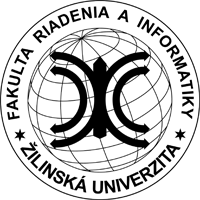
\includegraphics[scale=2,keepaspectratio=true]{./FRI_RGB_SK.png}
 % FRI_RGB_SK.png: 200x200 pixel, 300dpi, 1.69x1.69 cm, bb=0 0 48 48

\textsc{\newline\LARGE Žilinská univerzita v Žiline}\\[0.5cm]

\textsc{\Large Fakulta riadenia a informatiky}\\[0.5cm]

% Title
\HRule \\[0.4cm]
{ \huge \bfseries Analýza diferenčnej rovnice \\[0.4cm] }

\HRule \\[1.5cm]

% Author and supervisor
\begin{minipage}{0.4\textwidth}
\begin{flushleft} \large
\emph{Autori:}\\
Matejko Peter\\
Mudrák Ľuboš\\
Rehák Tomáš\\
Zárecký Martin\\
Boďa Michal\\
Kapusta Peter
\end{flushleft}
\end{minipage}
\begin{minipage}{0.4\textwidth}
\begin{flushright} 
\end{flushright}
\end{minipage}

\vfill

% Bottom of the page
{\large \today}

\end{center}
\end{titlepage}


\newpage

\tableofcontents



\newpage
\section{Zadanie}

V závislosti od hodnôt $ a \text{ a } b $
analyzujte riešenia danej diferenčnej rovnice\linebreak[4]
$x_{n+1}=\left(a+{\frac{b}{n}}\right)\,x_{n}$
kde $ a \text{ a } b $ sú reálne čísla, také, že $ a + b > 0$. Výsledky ilustrujte na jednoduchých príkladoch. 

Budeme skúmať dopady zmeny jednotlivých premenných $a$ a $b$ na riešenia danej diferenčnej rovnice.

\section{Definície}
\subsection{Pojem diferencia}

\begin{defin}
Je daný bod $x_{0}$ a číslo $h > 0$. Nech funkcia $y = f(x)$ je 
definovaná v bodoch $x_{0} \text{ a } x_{0} + h$. \textit{Diferencia funkcie }$f(x)$\textit{ v bode }$x_{0}$
je číslo $f(x_{0} + h) - f(x_{0})$. Značíme
$$\Delta f(x_{0}) = f(x_{0} + h) - f(x_{0})$$
\end{defin}
\subsection{Pojem diferenčná rovnica}
\subsubsection{Typy diferenčných rovníc}
\begin{defin}
(Diferenčné rovnice 1. typu) 
Nech pre všetky $x \in M$ je
definovaná funkcia $f(x, y, \Delta y, \Delta ^{2}y, \ldots, \Delta ^{k}y)$. Rovnica tvaru
$$f(x, y, \Delta y, \Delta ^{2}y, \ldots, \Delta ^{k}y) = 0 \text{ ,}$$
v ktorej neznámou funkciou $y = \varphi(x)$, nazývame diferenčnú rovnicu k-tého 
rádu a 1. typu definovanú v $M$.
\end{defin}

\textbf{\textit{Partikulárnym riešením}} tejto rovnice v $M$ nazveme každú funkciu
$y = \varphi(x)$, ktorá pre všetky $x \in M$ spĺňa danú rovnicu.

\paragraph{}
\textbf{\textit{Všeobecným riešením}} nazývame množinu všetkých partikulárnych
riešení.

\paragraph{}
\begin{defin}
(Diferenčné rovnice 2. typu)
Nech je pre všetky $x \in M$
definovaná funkcia
$$g(x, y_{x}, y_{x+1}, \ldots, y_{x+k})\text{, kde }y_{x+j} = \varphi(x + j) j = 0, 1, 2, \ldots, k\text{.}$$
\end{defin}

Rovnicu tvaru
$$g(x, y_{x}, y_{x+1}, \ldots, y_{x+k}) = 0\text{,}$$
v ktorej neznáma funkcia $y_{x} = \varphi(x)$, nazývaná \textit{diferenčná rovnica 2.typu}
definovaná v $M$. Ak je závislosť $g$ na $y_{x}$ a $y_{x+k}$ nekonštantná hovoríme,
že rovnica \textit{je k-tého rádu}. Riešenie rovnice v $M$ nazývame každú funkciu
$y_{x} = \varphi(x)$, ktorá pre všetky $x \in M$  spĺňa danú rovnicu. K tomu je nutné,
aby definičný obor funkcie $\varphi(x)$ obsahoval všetky $x \in M$ a taktiež body
$x + 1, x + 2, \ldots, x + k$.
\newpage
\subsubsection{Rekurentná formula}
Rekurentnú formulu vieme získať z diferenčnej rovnice vyjadrením $(n+k)$-tého člena pomocou $k$ predchádzajúcich členov rovnice.

\paragraph{}
Majme danú diferenčnú rovnicu: $$g(x, y_{x}, y_{x+1}, \ldots, y_{x+k}) = 0\text{.}$$

\begin{enumerate}
	\item Nech definičný obor tejto rovnice sú prirodzené čísla $ n = 1, 2, 3, \ldots$ a
		ďalej zaveďme všeobecnejšie označenie pre členy postupnosti: $ y_{n} =  a_{n}$,
		takže rovnicu vieme prepísať ako  $$g(n, a_{n}, a_{n+1}, \ldots, a_{n+k}) = 0\text{.}$$
		Predpokladajme, že túto rovnicu vieme jednoznačne rozriešiť vzhľadom k $ a_{n+k}$ :
		$$a_{n+k} = G(n, a_{n}, a_{n+1}, \ldots, a_{n+k-1})\text{,}$$
		kde $G$ je funkcia, ktorú sme dostali riešením pôvodnej rovnice.\linebreak[4]
		 Dostali sme vlastne všeobecný rekurentný vzorec pre postupnosť $a_{n}$,\linebreak[4] v ktorom je $(n+k)$-ty 				člen vyjadrený pomocou $k$ predchádzajúcich členov 
		$a_{n}, a_{n+1}, \ldots, a_{n+k-1}$ a premennej $n$.
	\item Pozrime sa na riešenie, keď máme vopred dané (ľubovoľné) čísla $ a_{1}, a_{2}, \ldots, a_{k}$.
		Vieme, že po dosadení členov do funkcie $G$ vypočítame jednoznačne člen
		$$a_{k+1} = G(1, a_{1}, a_{2}, \ldots, a_{k};)\text{,}$$ ďalším dosadením vypočítame
		$$a_{k+2} = G(2, a_{2}, a_{3}, \ldots, a_{k+1};)\text{atď.}$$
		Všeobecný $n$-tý člen $ a_{n} $ dostaneme vypočítaním elementárnej funkcie
		$n$ a daných $k$ prvých čísiel $ a_{1}, a_{2}, \ldots, a_{k}$. Táto funkcia je práve partikulárnym riešením 				diferenčnej rovnice s počiatočnými podmienkami $ a_{1}, a_{2}, \ldots, a_{k}$.	
\end{enumerate}

Touto druhou úvahou sa súčasne znovu potvrdzuje, že všeobecné riešenie rovnice $k$-teho rádu 
$a_{n+k} = G(n, a_{n}, a_{n+1}, \ldots, a_{n+k-1})$ má obsahovať
$k$ všeobecných konštánt, ktoré je možno si ľubovoľne zvoliť.

\newpage
\section{Vypracovanie}
\textbf{Popis našej rovnice}\newline
$x_{n+1}=\left(a+{\frac{b}{n}}\right)\,x_{n}$, kde $a,b \in R,\, a+b >0$. Ide o rekurentný vzorec pre postupnosť.\newline\newline
\textbf{Vypísanie prvých členov postupnosti}
\begin{spacing}{1.4}
\begin{tabbing}
\hspace{2cm}\=\kill
 $n=1$ :\> $x_{2}= (a+b)\*x_{1}$\\ 
 $n=2$ :\>  $x_{3}=(a+\frac{b}{2})\*x_{2}=(a+\frac{b}{2})(a+b)\*x_{1}$ \\ 
 $n=3$ :\>$x_{2}=(a+\frac{b}{3})\*x_{3}=(a+\frac{b}{3})\*(a+\frac{b}{2})(a+b)\*x_{1}$\\
 $n=4$ :\> $x_{2}=(a+\frac{b}{4})\*x_{4}=(a+\frac{b}{4})\*(a+\frac{b}{3})\*(a+\frac{b}{2})
 (a+b)\*x_{1}$\\ 
  $n=k-1$ :\> $x_{k}=(a+\frac{b}{k-1})\*x_{k-1}=(a+\frac{b}{k-1})\*(a+\frac{b}{k-2})\ldots(a+\frac{b}{2})\*(a+b)\*x_{1}$
\end{tabbing} 
\end{spacing}
 

\subsection{Triviálne riešenie}
Nech $x_{1}=0$.\newline
 Potom dostávame triviálne riešenie $x_{n+1} = 0$ a teda každý člen postupnosti bude mať hodnotu $0$. Ďalej, v našom vypracovaní, budeme predpokladať, že $ x_{1} > 0 $ a teda sa budeme 
zaoberať závislosťou od hodnôt $ a,b $.

\subsection{Všeobecné riešenie}
$x_{n+1}=\left(a+{\frac{b}{n}}\right)\*x_{n} \text{, } n \geq 1 \text{ a nech } a + {\frac{b}{n}} = f(n)$, potom
$x_{n+1}=f(n)\*x_{n}   $, kde $ n = 1 + k $, $ k = 0,1,2,... $
\begin{spacing}{1.3}
\begin{tabbing}
\hspace{1.5cm}\=\kill
$ x_{n}$\>$=f(n-1)\*x_{n-1}    $\\
$ x_{n-1}$\>$=f(n-2)\*x_{n-2}    $\\
$ x_{n-2}$\>$=f(n-3)\*x_{n-3}    $\\
\>\vdots \\
$ x_{n-(k-1)}$\>$=f(n-k)\*x_{n-k}    $
\end{tabbing} 
\end{spacing}
\noindent a teda $ x_{2} = f_{1}\*x_{1} $. 
%Kde počiatočná hodnota $x_{n}$ v bode $n=1$ je prvý člen postupnosti, teda zvolená konštanta.%

\subsection{Závislosť od hodnôt a, b}
Nech $ b=0 $,  $x_{1}>0$.\newline
Potom rovnica $x_{n+1}=\left(a+{\frac{b}{n}}\right)\*x_{n}$  nadobudne tvar  $x_{n+1}= a\*x_{n}$, 
teda každý ďalší člen postupnosti $x_{n+1}$ je $a$-násobkom predchádzajúceho člena  $x_{n}$.
Dosadením  $b=0$ teda vzniká z našej rovnice Geometrická postupnosť.
\newpage
Predpokladajme, že $ b=0 $ a $ a > 0 $, teda rovnica (*) má tvar $ x_{n+1} = a\*x_{n} $, čiže sa jedná o geometrickú postupnosť
$ x_{n} = a\*x_{n-1} $, kde $ a $ je koeficientom geometrickej postupnosti. 

V prípade, že $ a = 1 $ dostávame $ x_{n} = x_{n-1} $.
%Vraj nejake grafy%

Ďalej skúmajme prípad, kedy je $ a=0 $. Prvých pár členov vyzerá následovne: 
\begin{spacing}{1.6}
\begin{tabbing}
\hspace{1cm}\=\kill
$ x_{2}$\>$=b\*x_{1}    $\\
$ x_{3}$\>$=\frac{b}{2}\*x_{2} = \frac{b}{2}\*b\*x_{1}=\frac{b^{2}}{2}\*x_{1}   $\\
$ x_{4}$\>$=\frac{b}{3}\*x_{3} = \frac{b^{3}}{3!}\*x_{1}  $\\
\vdots \\
$ x_{n}$\>$=\frac{b^{n-1}}{(n-1)!}\*x_{1}    $\\
$ x_{n+1}$\>$=\frac{b^{n}}{(n)!}\*x_{1}    $\\
\end{tabbing} 
\end{spacing}
Čo sa podobá na Poissonove rozdelenie pravdepodobnosti. \\
Položme $ \sum\limits_{n=0}^\infty x_{n+1} = 1 $, potom $ 1=\sum\limits_{n=0}^\infty x_{n+1} = x_{1}\*\sum\limits_{n=0}^\infty \frac{b^{n}}{n!} = x_{1}\*e^{b}$ $ \Rightarrow $ $ x_{1} = e^{-b} $

Môžeme teda prehlásiť, že ak $x_{1}=e^{-b} $, potom riešením rovnice
$x_{n+1}=\left(a+{\frac{b}{n}}\right)\,x_{n}$ kde $a=0$, $b>0$
je Poissonovo rozdelenie $Po(\lambda)$ s parametrom $\lambda=b$.\\
Metódou matematickej indukcie sme teda dokázali, že $x_{n}\sim Po(\lambda)$, keďže každý ďalší člen $x_{n+1}\sim Po(\lambda)$.\\
%Koniec 246%

%247%

Ďalej skúmajme prípad, kedy $ a \in (0;1) $. Z pôvodnej rovnice teda :
\begin{spacing}{1.6}
\begin{tabbing}
\hspace{0.7cm}\=\kill 
$ x_{2}$ \> $=(a+b)\*x_{1} $\\
$ x_{3}$ \> $=(a + \frac{b}{2}) \* (a + b)\*x_{1} ) $\\
$ x_{4}$ \> $=(a + \frac{b}{3})\*x_{3}= (a + \frac{b}{3})\*(a + \frac{b}{2})\*(a + b)\*x_{1} $\\
\vdots \\
$ x_{n}$ \> $=(a + \frac{b}{n-1})\*(a + \frac{b}{n-2}) \ldots (a + \frac{b}{2})\*(a + b)\*x_{1}$\\
$ x_{n+1}$ \> $=(a + \frac{b}{n})\*(a + \frac{b}{n-1}) \ldots (a + \frac{b}{2})\*(a + b)\*x_{1}$\\
$ x_{n+1}$ \> $=\frac{a^{n}}{n!}\*(n + \frac{b}{a})\*(n-1 + \frac{b}{a}) \ldots (2 + \frac{b}{a})\*(1 + \frac{b}{a})\*x_{1}$,\\
\end{tabbing} 
\end{spacing}
kde $ x_{1} $ je prvým členom postupnosti. Vychádzajúc z $ a + b > 0 $ nech $ 1 + \frac{b}{a} = \alpha > 0$\\
$ x_{n+1} = \frac{a^{n}}{n!}\*(n+\alpha-1)\*(n+\alpha-2) \ldots (1+\alpha)\*\alpha\*x_{1}$\\\newpage
Po rozšírení pravej strany jednotkou v tvare $ \frac{(\alpha-1)!}{(\alpha-1)!} $ dostávame : \\
\begin{spacing}{2.2}
\begin{tabbing}
\hspace{0.7cm}\=\kill 
$ x_{n+1} = \frac{a^{n}\*(n+\alpha-1)!}{n!\*(\alpha-1)!}\*x_{1} $\\
$ x_{n+1} = a^{n}\* \dbinom{n+\alpha-1}{n}\*x_{1} $\\	%Pr alebo Po Kenny dobre ?%
$ x_{n+1} = \dbinom{n+\alpha-1}{n}\*(1-a)!^{\alpha}\*a^{n} = Pr(x = n) $,
\end{tabbing} 
\end{spacing}
kde $ x_{1} = (1-a)^{\alpha} \Rightarrow x_{1} = (1-a)^{1+\frac{b}{a}}$ 
%Koniec 247%%Teraz 248%
Môžeme teda povedať, že $ x_{n+1} \sim NB(2,9) $, číže $ x_{n+1}\sim NB (1+\frac{b}{a}; a) $,čo je negatívne binomické rozdelenie, pričom
$ a \in (0;1), a+b>0 \Rightarrow b \in (0;\infty), x_{1}=(1-a)^{a+\frac{b}{a}}$. Matematickou dedukciou je teda dokázané, že to platí aj pre 
$ x_{n} $.\\
%Koniec 248%%Zacina 244, ale to len prepisem, lebo neviem kam s tym%
%Keny mi prave povedal ze to tam nemam davat, co som napisal som zakomentoval 
%Ďalej budeme skúmať ďalší prípad, kedy $ a>0 $.\\
%Citujem "[21:28:33] Peter Kapusta: ten 244 tam nedavaj
%[21:28:42] Peter Kapusta: to zaro picovinu odfotil
%Z pôvodnej rovnice teda : 
%\begin{spacing}{1.6}
%\begin{tabbing}
%\hspace{0.7cm}\=\kill 
%$ x_{2}$ \> $=(a+b)\*x_{1} $\\
%$ x_{3}$ \> $=(a + \frac{b}{2}) \* (a + b)\*x_{1} ) $\\
%$ x_{4}$ \> $=(a + \frac{b}{3})\*x_{3}= (a + \frac{b}{3})\*(a + \frac{b}{2})\*(a + b)\*x_{1} $\\
%\end{tabbing} 
%\end{spacing} %
%Peto screen 46

Následne je potrebné sa zaoberať prípadom, keď $ a<0 $. Nesmieme však zabudnúť na podmienku $ a+b=0 $.
Predpokladajme, že existuje kladné celé číslo $ z $ také, že $ a + \frac{b}{z+1} = 0 $. V tomto prípade
platí, že pre všetky $ n\geq z+1  $ $ x_{n+1} = 0 $.
Kedže $ \frac{b}{n} (???) 0$ a $ b>0 $, $a + \frac{b}{n} \leq 0$ pre všetky dostatočne veľké $ n $. Ak $ z $ neexistuje,
potom zvolenie $ n $ je minimum tak $ a+\frac{b}{n} <0$, dostaneme $ x_{n+1} <0 $, čo je rozpor.
Môžeme teda písať $ z = -(1+\frac{b}{a}) $, potom :


\newpage
\section{Záver}


\begin{thebibliography}{9}
\bibitem{pra}{\em Prágerová, A.:}
               {\bf Diferenční rovnice.}
           Polytechnická knižnice, Praha 1971.
\end{thebibliography}

\end{document}
